\subsection{HexGame et stratégie gagnante}

Au Hex, pour toutes les tailles de plateaux il existe une stratégie gagnante théorique pour le joueur qui commence.
Cependant, celle-ci n'est pas connue pour la plupart des tailles de plateaux. En effet, celle-ci demande une connaissance totale de toutes 
les parties possibles, ce qui n'est pas calculable en temps realiste.

\subsubsection{Stratégies gagnantes et arbre du jeu}
Modélisons le jeu du Hex à l'aide d'un arbre représentant toutes les parties possibles, L'arbre commence avec la position 
initiale, un plateau vide. De cette racine partent autant de branches qu'il n'y a de possibilités pour 
le premier coup du premier joueur. On réitère cette action pour chaque nœuds jusqu'à tomber sur des positions gagnantes pour l'un des deux joueur
%faire exemple
\begin{figure}[!htb]
    \begin{center}
        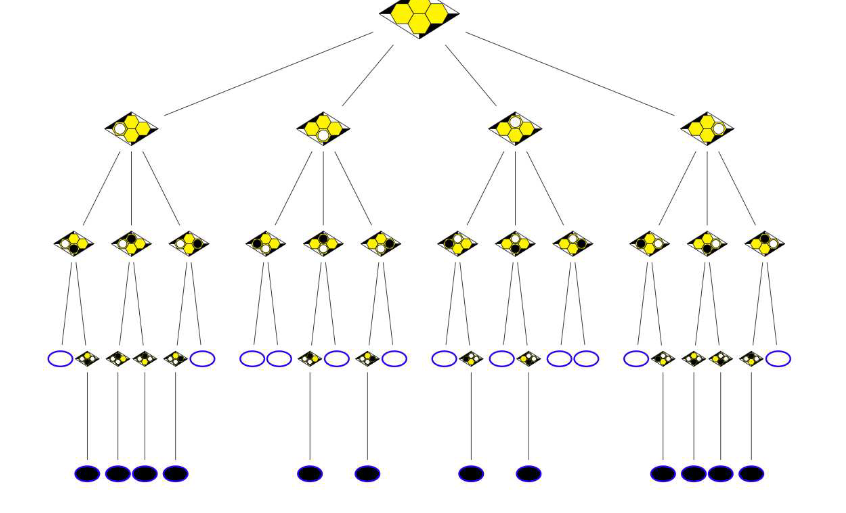
\includegraphics[width=0.4\textwidth]{root/strategie_gagnante.png}
    \end{center}
    \caption{Exemple pour un plateau $2\times2$}\label{fig:strategie_gagnante}
\end{figure}

L'arbre va nous aider à nous convaincre qu'il y a bien une stratégie gagnante pour l'un des deux joueurs. 
Le principe consiste à colorier tous les nœuds de l'arbre en blanc ou en noir, chaque
nœud colorié correspondant à une position à partir de laquelle le joueur de la couleur correspondante
possède une stratégie gagnante. 
Nous commençons par colorier en blanc les feuilles représentant une fin de
partie gagnée par les blancs, en noir celles correspondant à la victoire du joueur noir.
Le reste du coloriage se fait progressivement. À un moment donné, on veut attribuer une couleur
à un nœud qui n'en a pas encore, mais dont toutes les branches descendantes mènent à des nœuds
déjà coloriés. Supposons que ce nœud représente une position à partir de laquelle c'est aux blancs de
jouer. Si au moins l'une des branches issues du nœud mène à un nœud blanc, alors on colorie le nœud
en blanc. Dans le cas contraire, c'est-à-dire si toutes les branches mènent à des nœuds coloriés en
noir, on le colorie en noir. On procède de façon symétrique si c'est aux noirs de jouer.
De cette manière nous sommes assurés de remplir l'abre de nos couleurs jusqu'à la racine. 
Ainsi, la racine possède une stratégie gagnante.


\subsubsection{Remarques}
-On voit que pour un plateau de dimension $2\times2$, l'arbre de tous les possibles possède déjà 24 feuilles et 52 branches.
Il est calculé que pour un plateau de taille $11\times11$, le nombre de feuilles de l'arbre est
approximativement $10^{98}$, et le nombre de positions totales que peut prendre le jeu est de $2.4\times10^{56}$.
Donc en pratique, utiliser cette technique pour trouver la stratégie gagnante n'est pas possible.

-Il est aussi possible d'appliquer ce genre de raisonnement à d'autres jeux combinatoires abstraits pour essayer de
prouver l'existence d'une éventuelle stratégie gagnante.

-Enfin, on remarque que cette façon de faire ressemble à l'algorithme MinMax s'il avait une profondeur de recherche
infinie.


\subsubsection{Le premier joueur gagne à tous les coups}
On a vu que il existe une stratégie gagnante, mais on ne sait pas pour quel joueur est le gagnant. Dans ce paragraphe nous allons
prouver que le joueur 1, s'il joue parfaitement, gagne à tous les coups.

Puisque les matchs nuls sont impossibles, nous pouvons conclure que soit le premier, soit le deuxième joueur possède une stratégie
gagnante. Supposons maintenant que le deuxième joueur ait une stratégie gagnante.

Le premier joueur adopte alors la stratégie suivante : il effectue un mouvement arbitraire. Ensuite, 
il joue en utilisant la supposée stratégie gagnante du deuxième joueur mentionnée ci-dessus. Si,
en jouant cette stratégie, il doit jouer sur la case où un mouvement arbitraire a été fait, il effectue
un autre mouvement arbitraire. De cette manière, il suit la stratégie gagnante tout en ayant toujours une pièce
supplémentaire sur le plateau.

Cette pièce supplémentaire ne peut pas interférer avec l'imitation par le premier joueur de la stratégie gagnante.
En effet, une pièce supplémentaire pour le joueur 1 n'est jamais un désavantage. Par conséquent, le premier joueur peut
gagner.

Comme nous avons maintenant contredit notre hypothèse selon laquelle le deuxième joueur aurait une stratégie gagnante,
nous concluons qu'il n'y a pas de stratégie gagnante pour le deuxième joueur.

Par conséquent, il existe une stratégie gagnante pour le premier joueur.